\section{Process Management}

% Section overview.
In this section, we take a closer look in the process management
subsystem. We start by first presenting the process structure
itself; then highlighting how process scheduling and switching
happens; and finally discussing the most important mechanisms
exported by this subsystem.

\subsection{The Process Structure}
\label{subsection: the process structure}

	% Process abstraction overview.
	A process is an abstraction of a running program. It depicts the
	memory core, opened files, execution flow, access permissions,
	current state and every other relevant information about a program.
	Table \ref{table: process structure} outlines the (simplified)
	structure of a process in Nanvix. The information about all
	processes is kept in a kernel table, named the process table, and it
	is globally visible to all subsystems.

	\begin{table}[h]
	\footnotesize
	\centering
	\caption{Simplified structure of a process in Nanvix.}
	\label{table: process structure}
	\begin{tabular}{l l l}
		\toprule
		Category & Field & Description \\
		\midrule
		\multirow{3}{*}{\specialcell{Context Switch\\Information}} & \texttt{kesp}   & Kernel Stack pointer \\
																   & \texttt{kstack} & Kernel Stack         \\
																   & \texttt{intlvl} & Interrupt Level      \\
		\midrule
		\multirow{3}{*}{\specialcell{File System\\Information}} & \texttt{pwd}    & Current Working Directory \\
																& \texttt{ofiles} & Opened Files              \\	
																& \texttt{tty}    & Output Terminal Device    \\
		\midrule
		\multirow{2}{*}{\specialcell{General\\Information}} & \texttt{status} & Exit status                                          \\
															& \texttt{pid}, \texttt{gid}, \texttt{uid} & Process, group and user IDs \\
		\midrule
		\multirow{2}{*}{\specialcell{Memory\\Information}} & \texttt{pregs} & Code, data, stack and heap segment regions \\
														   & \texttt{pgdir} & Page directory       \\
		\midrule
		\multirow{4}{*}{\specialcell{Scheduling\\Information}} & \texttt{state}    & Current state       \\
															   & \texttt{counter}  & Remaining quantum   \\
															   & \texttt{nice}     & Priority adjustment \\	
															   & \texttt{priority} & Priority            \\
		\midrule
		\multirow{2}{*}{\specialcell{Signal\\Information}} & \texttt{received} & Received signals \\
														   & \texttt{handler}  & Signal handlers  \\
		\midrule
		\multirow{2}{*}{\specialcell{Timing\\Information}} & \texttt{utime} & User CPU Time   \\
														   & \texttt{ktime} & Kernel CPU Time \\
		
		\bottomrule
	\end{tabular}
	\end{table}

	% Process table maintenance.
	The process management subsystem maintains the process table:
	whenever a new process is created, a new entry is added to it; and
	when a process terminates, the corresponding entry is erased.
	However, it is worthy to point that each subsystem is in charge of
	maintaining their own fields in the process structure.  For
	instance, the memory management subsystem is the one that fills up
	information regarding the segment regions and page directory,
	whereas the file system keeps track of the current working directory
	and opened files fields.

	% Process states.
	A process is created whenever a user launches a program or the
	system itself spawns a new daemon. After that, the new process goes
	through a complex lifetime before it terminates, as it is shown in
	Figure \ref{figure: states of a process in nanvix}.  Initially this
	new processes is ready to execute (\textit{Ready}), and it is
	eventually selected to run by the scheduler. At this moment, the
	process resumes back its execution in kernel land (\textit{Kernel
	Running}) and jumps to userland (\textit{User Running}). There, the
	process performs some computation, and when a software/hardware
	interrupt occurs the process may either: (i) get preempted if it
	runs out of quantum time (\textit{Ready}); (ii) block waiting for a
	resource (\textit{Sleeping}); or (iii) suspend execution until the
	receipt of a signal (\textit{Waiting}).  Either way, the process
	later resumes its work, and loops back on these states.  When the
	process finally gets its job done, or it somehow crashes, it
	terminates and becomes a zombie process (\textit{Zombie}). A zombie
	process awaits to gets all resources assigned to it to be taken away
	by the kernel, and then it is turned in a dead process
	(\textit{Dead}).

	\begin{figure}[t]
		\centering
		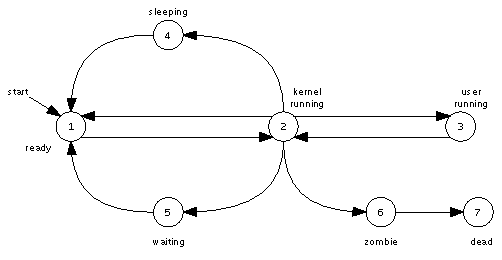
\includegraphics[width=\linewidth]{img/process-states}
		\caption{States of a process in Nanvix.}
		\label{figure: states of a process in nanvix}
	\end{figure}

\subsection{Process Scheduling and Switching}

	% Process scheduling overview.
	Several processes may be active in the system, but only one can
	be running at a time\footnote{Nanvix does not support
	multiprocessor systems, thus processes are indeed not running in
	parallel.}. The scheduler chooses which process to run next
	whenever the running process gets preempted or blocks. In user
	mode, that happens when the running process runs out of quantum
	and gets preempted by the kernel, or else when it issues a
	system call. In kernel mode on the other hand, scheduling occurs
	only when the running process voluntarily relinquishes the
	processor and goes wait for a resource to be released.

	% Scheduling policy.
	The scheduler (Figure \ref{figure: scheduler}) uses a priority
	based criteria to choose the next process to run, with processes
	with higher priorities being scheduled to run before those with
	lower priorities\footnote{Nanvix adopts the Unix's priority
	system, in which lower values mean higher priorities.}.
	Processes with equal priorities are chained in a queue and are
	selected in a round-robin fashion.

	% Priorities of a process.
	The priority of a process changes over the time and it is given
	by the sum of three numbers: base priority, dynamic priority and
	nice value. The base priority is assigned by the kernel itself
	and changes as the process sleeps and wakes up from resource
	queues, and leaves the kernel or enters it. The dynamic priority
	is increased by the scheduler as the process waits longer in the
	ready queue. Finally, the nice value is adjusted by the users,
	exporting them a mechanism to control which processes are more
	priority over others.

	% Process switching.
	Once the scheduler chooses which process to run next, the
	process management subsystem performs the context switching
	operation. It first pushes the contents of all machine registers
	in the kernel stack. Then, it instructs the memory management
	unit hardware to switch to the address space of the selected
	process. Finally, the state of the machine registers are
	restored from the kernel stack of the selected process. The
	context switching operation is machine dependent and it is
	actually carried on by the hardware abstraction layer.

	\begin{figure}[t]
		\centering
		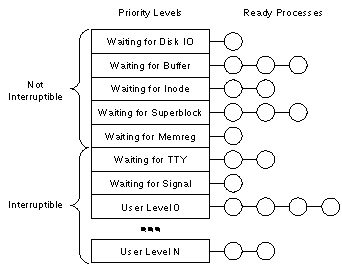
\includegraphics[scale=1.4]{img/scheduler}
		\caption{Scheduler queues.}
		\label{figure: scheduler}
	\end{figure}

\subsection{Process Creation and Termination}

	% Process creation.
	In Nanvix, processes are created through the \texttt{fork()}
	system call. This call instructs the process management
	subsystem to create a new process that is an exact copy of the
	calling process. The primal process is called parent and the new
	process is called child, and they have the same code, stack and
	data segments, opened files and execution flow, differing only
	differ in their ID number. The \texttt{fork()} system call is a
	complex and expensive operation, and in order to get it done the
	process management subsystem heavily interacts with the memory
	management system and the file system.

	% fork() in a nutshell.
	To create a process, the kernel first looks for an empty slot in
	the process table, to store there the information about the
	process. Then, an address space for the process is created: page
	tables are initialized, the kernel code and data segments are
	attached to the process' core, and a kernel stack for the
	process is created. After that, the kernel duplicates every
	memory region of the parent process and attaches them to the
	address space of the child process. In this operation,
	underlying pages are not actually copied, but they are rather
	linked and copied on demand. This technique, called
	copy-on-write, greatly speeds up the \texttt{fork()} system
	call, and it is covered in Section \ref{subsection: the virtual
	memory and paging systems}. Then, when the address space of the
	new process is built, file descriptors for all opened files are
	cloned, and every other information is handcrafted. Finally, the
	process management system marks the child process as new, so
	that the scheduler can properly handles this situation, and
	places it in the ready queue for later execution.

	% Process termination.
	The process then performs some computation and undergoes through
	a complex lifetime, which we depict in Section \ref{subsection:
	the process structure}. When the process finally finishes its
	job it invokes the \texttt{exit()} system call to terminate.
	This call orders the process management subsystem to actually
	kill the process and release all resources that are assigned to
	it.

	% exit() in a nutshell.
	To do so, several steps are involved. First, the kernel masks
	out signals and closes all files that are still opened. After
	that, all child processes of the process that is about to
	terminate are assigned to a special process, called
	\texttt{init}\footnote{\texttt{init} is a daemon process whose
	job is to spawn the logging processes.}. This ensures that no
	process becomes orphan, and thus become unreachable by signals
	(see Section \ref{subsection: process synchronization and
	communication}). Then, the kernel detaches all memory regions
	from the dying process and marks it as a zombie. At this moment,
	the dying process still has an address space and a slot in the
	process table, and the kernel has no way to wipe off these
	information. Therefore the dying process hands out this task to
	the parent process, and sends a death of child
	(\texttt{SIGCHLD}) to it. This signal cannot be blocked or
	ignored, and it is eventually handled by the corresponding
	parent process. When that happens, the parent process destroys
	the address space of its zombie child process, and marks the
	corresponding slot in the process table as not used.

\subsection{Process Synchronization and Communication}
\label{subsection: process synchronization and communication}

	% Process synchronization.
	In Nanvix, processes may cooperate to one another to accomplish
	a common goal. To enable this, the kernel provides three
	synchronization primitives, so that processes can work together
	without messing up each other's job: \texttt{sleep()},
	\texttt{wakeup()} and \texttt{wait()}.

	% sleep() and wakeup() in a nutshell.
	When running in kernel land, processes often need to acquire and
	later release resources, such as slots in the system's tables
	and some temporary memory. The \texttt{sleep()} and
	\texttt{wakeup()} routines are used in these situations to avoid
	race conditions in kernel land. The former puts the calling
	process to wait in a chain; whereas the later causes all
	processes that are sleeping in a chain of processes to be moved
	to the ready-to-execute scheduling queue. These routines support
	two different sleeping states: one that is interrupitible by the
	receipt of signals, and another that is not. Thanks to this
	mechanism, users can interact with foreground processes, such as
	those that read/write to the terminal.

	% wait() in a nutshell.
	In userland, processes may coordinate their activities by
	calling the \texttt{wait()} system call. This call causes a
	process to block until one of its child process terminates. When
	such event happens, the parent process is awaken and the exit
	status of the terminated child is made available to it. This
	information can be later parsed by the parent process, so that
	it can known why exactly its child process has terminated and
	properly handle the situation.

	% Process communication.
	These three mechanisms enable processes to synchronize their
	activities and friendly work together towards a common goal.
	Notwithstanding, processes also have to somehow be able to
	communicate with one another to exchange valuable information
	about their work progress. Nanvix offers two main mechanisms to
	do that: signals and pipes.

	% Signals in a nutshell.
	Signals are short messages that processes can send/receive
	asynchronously. They are mainly used to notify about the
	occurrence of interesting events, such as that a process has to
	be killed, a remote terminal has hangup and a breakpoint has
	been reached. The process management subsystem exports two
	system calls to deal with signals: \texttt{signal()} and
	\texttt{kill()}. The former allows a process to actually control
	how signals shall be handled. A process can either choose to
	ignore a signal, and not be notified at all about it, or else
	handle a signal, by registering a callback function that will do
	the job. The \texttt{kill()} system call on the other hand,
	allows a process to raise a signal, either to another process or
	to itself. Additionally to these system calls, the kernel also
	provides a system call, named \texttt{pause()}, which allows a
	process to wait for the receipt of a signal. Signals are
	implemented by having the kernel to instrument the user stack,
	when a signal is send. The kernel carefully inserts hooks to the
	registered signal handler in the stack, and when the process
	leaves the kernel, it transparently executes the signal handler
	function (Figure \ref{figure: signal stack}).

	% Pipes in a nutshell.
	Signals are useful for exchanging small amount of information.
	However, if processes want to carry on more verbose
	conversations, they can use pipes instead. A pipe is a virtual
	file that serves as a dedicated communication channel between
	two processes. At one end of the pipe, a writer process puts
	data on the pipe, and at the other end a reader process takes
	data out from it. Processes can open pipes through the
	\texttt{pipe()} system call, and after that they can read/write
	data to it by using the \texttt{read()} and \texttt{write()}
	system calls, as they would normally do. In all these
	operations, data transfers take place entirely in memory, with
	the kernel borrowing a page frame from the kernel page pool and
	pinning it in memory. Additionally, the kernel handles the
	required producer-consumer synchronization with the help of the
	\texttt{sleep()} and \texttt{wakeup()} routines.

	\begin{figure}[b]
		\centering
		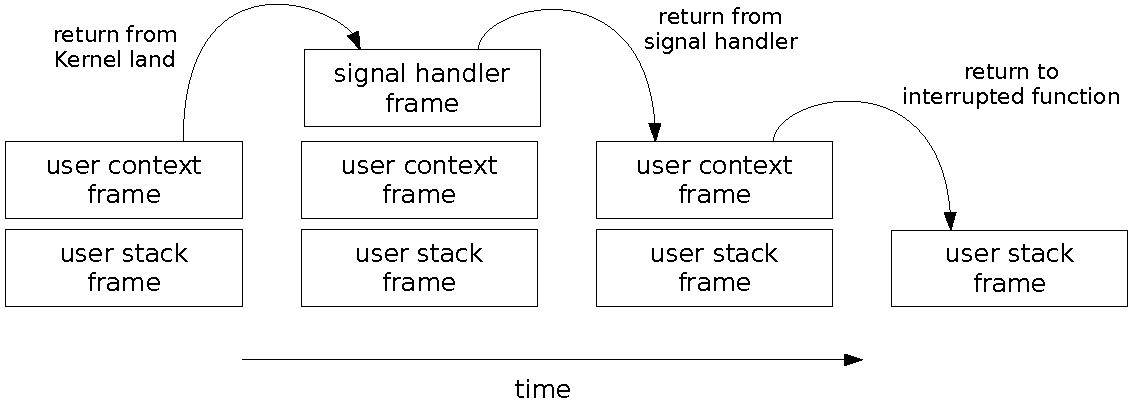
\includegraphics[scale=0.55]{img/signal-stack}
		\caption{Signal stack.}
		\label{figure: signal stack}
	\end{figure}

